% ====================================================================
%+
% SECTION:
%    section-name.tex  % eg lenstimedelays.tex
%
% CHAPTER:
%    chapter.tex  % eg cosmology.tex
%
% ELEVATOR PITCH:
%    Explain in a few sentences what the relevant discovery or
%    measurement is going to be discussed, and what will be important
%    about it. This is for the browsing reader to get a quick feel
%    for what this section is about.
%
% COMMENTS:
%
%
% BUGS:
%
%
% AUTHORS:
%    Phil Marshall (@drphilmarshall)  - put your name and GitHub username here!
%-
% ====================================================================

\section{Mapping the Milky Way Halo}
\def\secname{MW_Halo}\label{sec:\secname} % For example, replace "keyword" with "lenstimedelays"

\noindent{\it Kathy Vivas, Colin Slater, David Nidever, Beth Willman}  % (Writing team)

The study of the Halo of the Milky Way is of the most importance not only to understand
the formation and early evolution of our own galaxy, but also to test 
test current models of hierarchical galaxy formation. 
LSST will provide an unprecedented combination of
area, depth, multi-band, multi-epoch information for pursuing detail studies
of the structure of this old Galactic component. We focus here in three
specific projects that can be pursued with LSST. We suggest metrics and figure of merits that can
be calculated in order to quantify the feasibility of the projects under different
observational strategies. We expect more projects will join later.

RR Lyrae stars have been known for several decades as excellent tracers
of the halo population. They are not only old stars ($>10$ Gyrs) but they are
also excellent standard candles that allow to build 3-dimensional maps. 
The halo of the Milky Way has been now surveyed in a very large extension up to 
$\sim 60-80$ kpc from the Galactic center \citep[][among others]{drake13a,drake13b,zinn14,torrealba15}. 
Beyond that, the halo is
mostly uncharted territory.
From these RR Lyrae surveys, we have learned that the halo is filled with substructures
which are usually interpreted as debris from destroyed satellite galaxies. The smooth 
component of the RR Lyrae distribution is well described
with a power-law of the mean number density of RR Lyrae stars as a function of
galactocentric distance, which gets steeper after $\sim 30$ kpc \citep{zinn14}. 
Thus, beyond $\sim 60$ kpc, few field RR Lyrae stars are expected. However, we presume that 
any RR Lyrae star beyond this distance may be part of either debris material or distant
satellite galaxies of low luminosity that have been escaped detection until now \citep{sesar14,baker15}. 
LCDM models predict debris as far as $0.5$~Mpc from the galactic center
This is the territory that will be explored by LSST.

Similarly, red giant stars can be used to trace the structure of the halo up to large
distances. They have the advantage 
of being bright and numerous stars.

Fainter than these two tracers, main sequence stars stand up as a tool for studying
the Halo. They are the most numerous type of stars available and statistical studies 
are possible. Using the technique of photometric metallicities \citep{ivezic08}, 
the Sloan Digital Sky Survey (SDSS) provided unprecedented maps of the metallicity distribution up to  $\sim 10$ 
kpc from the Galactic center, unveiling not only the mean metallicity distribution 
of the halo but also, sub-structures within the halo. This kind of works will be extended
to the outermost parts of the Galaxy with LSST data.


% --------------------------------------------------------------------

\subsection{Target measurements and discoveries}
\label{sec:\secname:MW_Halo_targets}

The three projects just described require the discovery and/or measurement of the following 
type of objects:

\begin{itemize}

\item RR Lyrae stars: These are bright horizontal-branch variable stars with
periods between 0.2 to 1.0 days and large amplitudes, particularly in the bluer 
bandpasses (g amplitudes $0.5 - 1.5$~mag). \citet{2012AJ....144....9O} made an intensive
search for RR Lyrae stars in simulated LSST data and reached to the conclusion 
that this type of stars can be recovered to distances $\sim 600$ kpc. A similar procedure
can now be performed using MAF and current cadence scenarios.
Chapter \ref{chp:variables} discusses the discovery metrics for variable stars 
including RR Lyrae stars. However, optimal recovery may involve more complex metrics
involving the simultaneous use of multi-band time series \citep{vanderplas15,vivas16}.
Besides the recovery of the variable stars, a particularly valuable measurement to track 
for studies in the halo is the infrared mean magnitudes z and y since they provide the 
most accurate way to obtain distances \citep{caceres08}. 

\item Main sequence stars: lacking any distinguishable variability, the
challenge in selecting a large and clean sample of main sequence stars comes
from tremendous number of small and nearly-unresolved galaxies present at
faint magnitudes. Precise star/galaxy separation is thus the limiting factor
on the useful depth of the main sequence sample. In addition to identifying
dwarfs, using dwarfs to map the metallicity distribution of the halo requires
precise u-band data, since it exhibits the strongest metallicity dependence of
the LSST filters.

\item Red Giants: due to their intrinsic luminosity red giants will be sample
a far deeper volume than main sequence stars at similar apparent magnitudes,
but they must first be identified and separated from the very numerous main
sequence stars present in the field. A gravity-sensitive photometric index can
be used for separating efficiently giants from dwarfs. The u magnitude
is an essential ingredient in this process and it is necessary to follow-up
the behavior of the u limiting magnitude under different observational
strategies. Figure~\ref{fig-MW-giants} shows the distance that can be reached 
by M giants of different metallicities assuming a limiting magnitude in the u band of
26.0. 

\end{itemize}

\begin{figure}
\begin{center}
  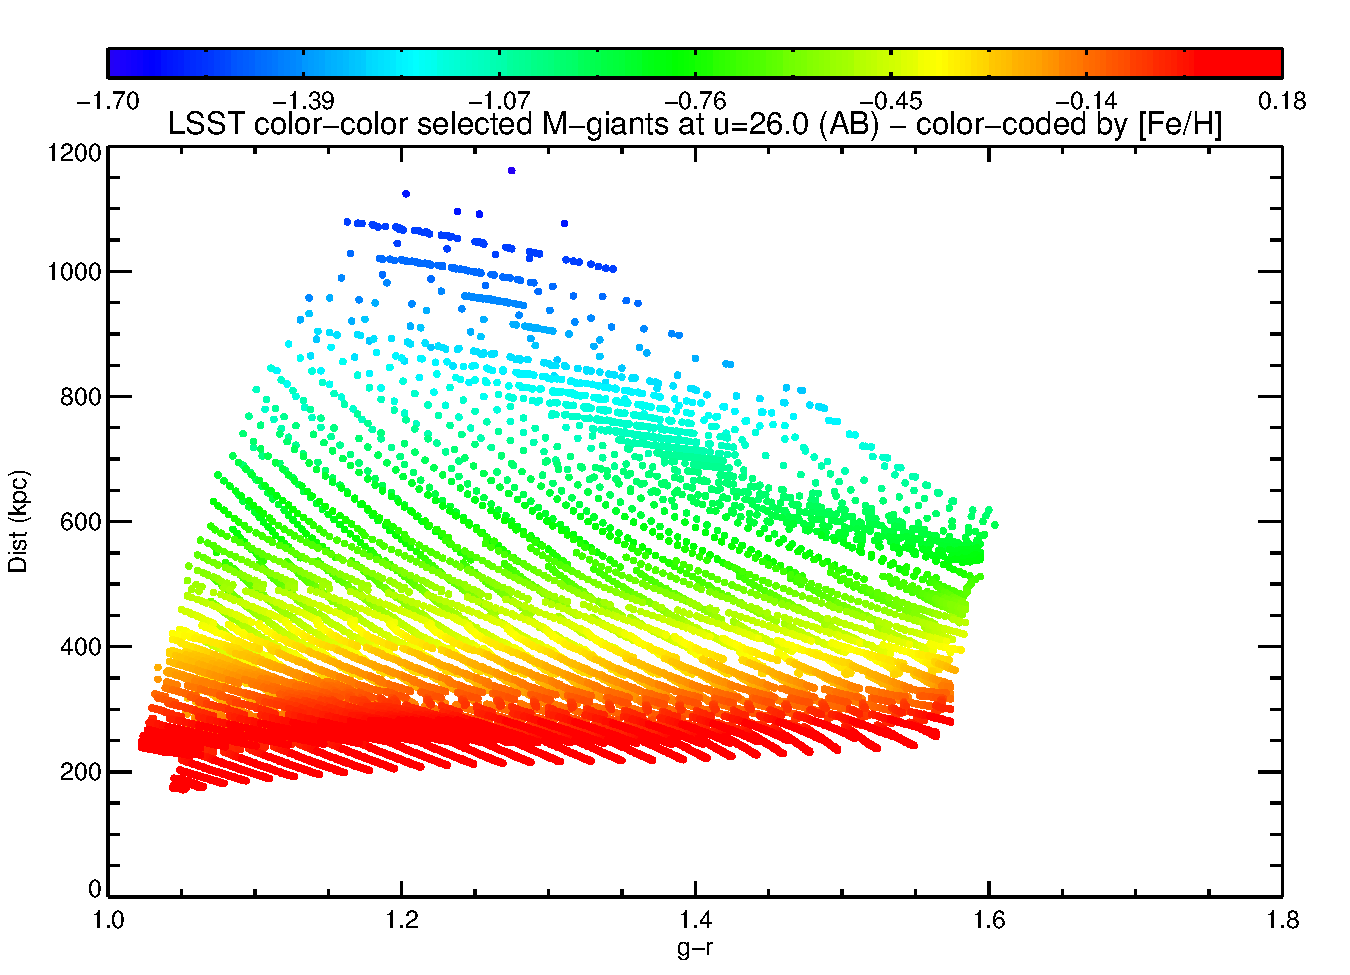
\includegraphics[scale=0.5]{./figs/milkyway/lsst_mgiants_grdist.pdf}
  \caption{Distance to which red giant stars can be identified in the galactic halo asuuming a limiting magnitude
  of u=26.0. The color code scales with the metallicity of the stars. More metal-poor stars can be 
  detected to farther distances. \label{fig-MW-giants}}
\end{center}
\end{figure}


% --------------------------------------------------------------------

\subsection{Metrics}
\label{sec:\secname:MW_Halo_metrics}

\textbf{Star-Galaxy Separation:} For main sequence stars, the useful depth of
the survey will likely not be the photometric detection limit but will instead
be set by the ability to differentiate stars from unresolved background
galaxies. Towards faint magnitudes the contamination by galaxies worsens
significantly for several reasons: the number of galaxies is rising
substantially, the angular size of galaxies is shrinking, and our ability to
distinguish stars from marginally resolved galaxies diminishes for faint
sources simply due to photon statistics. While the fundamental properties of
the contaminant sources is beyond our control, our ability to reject these
sources depends on survey parameters such as the distribution of seeing across
visits and the depth of these visits.

We are currently in the process of developing a metric that will estimate our
ability to separate stars and galaxies for any observation depth and seeing
conditions. This requires both an understanding of how images of a source are
measured and classified as either a star or galaxy, and how the population of
stars and galaxies vary in number and size (for galaxies) with depth. Our model
uses the distribution of galaxies in size and number, derived from HST COSMOS
observations, along with a fully Bayesian model decision formalism to compute
the expected completeness and contamination in star-galaxy separation.
Computationally for each position in the survey footprint we interpolate the
results from that work on a grid in seeing, galaxy size, and coadd depth, then
integrate over the distribution of galaxy sizes. This modeling process is
currently being verified against existing surveys, and will be incorporated into
the observing strategy study at a later date.

This is a diagnostic metric and some of the higher level metrics described below 
will depend on this one.

\textbf{Distance to the farthest RR Lyrae stars:} This metrics involves the ability to
recover an RR Lyrae star as a function of its distance. An RR Lyrae star may be
considered as recovered if its period and amplitude are within 10\% of their real values.
The procedure followed by \citet{2012AJ....144....9O} is a good example on how this can be
achieved. They built a large number of synthetic light curves spanning the properties of
known RR Lyrae stars and {\sl observed} them with the cadence given by the OpSim runs
available at that time. An improvement over this previous work should include the use
of simultaneous multi-band information to recover periods \citep[e.g.,][]{vanderplas15,vivas16}.

However, a first look into this problem using MAF can be achieved
by simplifying the procedure and only test if a star with period 0.55 days (the mean period for
RR Lyrae stars) can be recovered by metrics already available in MAF.
Then, distance can be calculated using the mean magnitude of the recovered RR Lyrae stars 
(in the more IR photometrics bands) and the interstellar extinction at that point of the sky (maps are available 
now in MAF).  Output of this metric should be the largest distance that can be measured with a 10\% precision
at which certain percentage of RR 
Lyrae stars (eg. 80\%) can be recovered by LSST. It is expected that the results 
of this metric at low galactic latitudes will be largely dependent on the chosen observational 
strategy (how sparse will the cadence be  in the galactic plane).

A reasonable Figure of Merit for this sub-project is the volume of the halo within RR Lyrae stars 
can be recovered. Similarly, another Figure of Merit is the fraction of the Galactic thick disk's volume that can be 
traced by RR Lyrae stars.

\textbf{Distance to the farthest main sequence stars and giant stars:} Being non-variable objects
the metrics for these objects are somewhat simpler and requires the determination of the limiting
magnitude (in u band) for which galaxy/star separation is reliable to certain level. In these cases, distances
depend on metallicity. Then, a figure of
merit is the volume of the halo mapped with stars within certain metallicity range. 


% --------------------------------------------------------------------

\subsection{OpSim Analysis}
\label{sec:\secname:MW_Halo_analysis}

Table \ref{tab_SummaryMWHalo} summarizes the science Figures of Merit
for the Milky Way Halo science cases for LSST. OpSim analysis for this
Section will be summarized in that Table; at the present date (April
2016) placeholder rows are given for the FoM's. Input from the readers
is welcome!

%%% SUMMARY TABLE FOR THIS SUBSECTION

\begin{table}
  \begin{tabular}{l|p{6cm}|c|c|c|c|p{5cm}}
    FoM & Brief description & {\rotatebox{90}{\opsimdbref{db:baseCadence} }} & {\rotatebox{90}{\opsimdbref{db:opstwoPS} }} & {\rotatebox{90}{future run 1}} &  {\rotatebox{90}{future run 2}} & Notes \\
    \hline
    1.1. & \footnotesize{Survey volume to RR Lyraes}      & - & - & - & - & \footnotesize{Volume within which the distance to a template RR Lyrae star can be estimated to 10\% uncertainty.} \\
    1.2. & \footnotesize{Survey volume to Main Sequence tracers} & - & - & - & - & \footnotesize{(Including star-galaxy separation)} \\
    1.3. & \footnotesize{Survey volume to Red Giants} & - & - & - & - & - \\
%    2.1. & \footnotesize{Completeness of metallicity sub-structure recovery as a function of distance} & - & - & - & - & \footnotesize{Over all three tracer populations?} \\ 
%    3.1. & \footnotesize{Uncertainty and bias in age distribution parameterization of the main Halo population} & - & - & - & - & - \\
%    3.2. & \footnotesize{Uncertainty and bias in the population fraction identified correctly with each halo component} & - & - & - & - & \footnotesize{Some overlap with Halo astrometry FoM?} \\
\end{tabular}
\caption{Summary of figures-of-merit (FoMs) for the Galactic Halo science cases. The best value of each FoM is indicated in bold. Runs \opsimdbref{db:baseCadence} and \opsimdbref{db:opstwoPS} refer to the Baseline and PanSTARRS-like strategies, respectively. See Section \ref{sec:MW_Halo}.}
\label{tab_SummaryMWHalo}
\end{table}


% --------------------------------------------------------------------

%\subsection{Discussion}
%\label{sec:\secname:MW_Halo_discussion}

%Discussion: what risks have been identified? What suggestions could be
%made to improve this science project's figure of merit, and mitigate
%the identified risks?


% ====================================================================

\navigationbar
